\chapter{Goals} \label{chap:Goals}




% \section{System Architecture}
% \begin{figure}[!b]
% 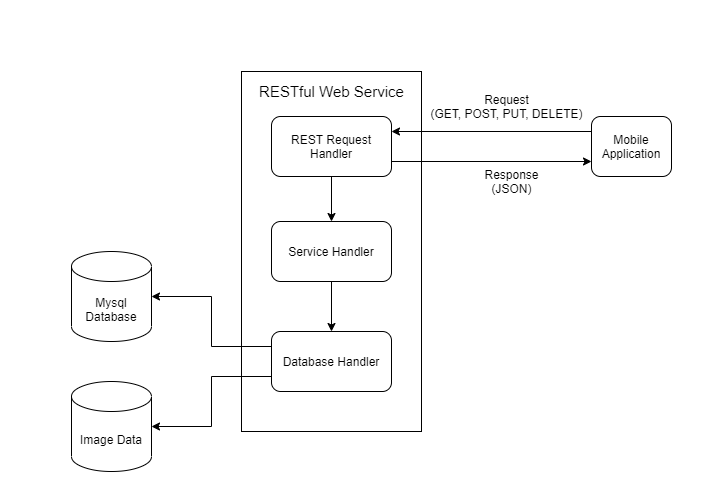
\includegraphics[width=14cm]{Images/App/System_Design.png}
% \caption{System Architecture Design}
% \end{figure}

% At first, this application has two system options: One that requires no additional server to run, all of the service is installed locally on the user's devices. Since our core service, the diagram detection algorithm is written with C++ then it can run on any system. Then we intended to build an application system that can handle the whole process of pre-processing image and create the result without the internet connection. However, as our target is to support all the device that runs android 7.0 and above (that means all smartphones manufactured from 2016 to present and some of them can be older), it could lead to a performance problem because many of them were outdated 2 or 3 years. Another issue is sharing between users will have to be dependent on a third-party service. Which is not convenient and may lower the user experience.

% The second one is to build a REpresentational State Transfer Application Programming Interface (REST API) service, run on a node.js server, which will handle all the requests sent by users and store all the data on a system database so that users can now store all of their data online without worry about their phone internal storage. the web server can be divided into three main components: Request handler, Service handler and Database handler. All of the detection and management will be mainly process in the second component, then all of the data will be transfer to a My SQL database, including user data and diagram file. However, all of the uploaded images that sent to the server to process will be then stored in the image storage separated from main database for additional data to improve detection algorithm in the future. The downside of this approach is now in order to use the app, the application has to be stably connected to the internet to make any changes to their data (create, edit, remove,...). Another challenge for us is to optimize the server so it can process a lot of access at the same time.



% \section{Framework}
% \subsection{Flutter}
% Flutter is a user interface toolkit developed by Google for building beautiful, natively compiled applications for mobile, web, and desktop from a single code base \cite{57}. Dart is the main programming language used in Flutter.

% One of the most beloved of Flutter that finally made it the framework we use in this thesis is it can create great and modernized user interfaces that really suit our design code for this project: simplistic but easy to use. Although the result can be used to build both android and iOS (potentially web) applications, the target of this project is to focus on one platform at first and continue to grow in the future. Despite being a recently released framework built for mobile development, Flutter provides a lot of features that speed up the development process as well as a growing community to share and learn.

% However, there is also a downside of it, since it was born to build an application that can run on many different platforms, the performance loss is inevitable compared to natively built applications. Even though Flutter has been optimized and guarantee 60 frames per second but it still heavily depends on developers to make good use of available performance resources. Another one is the application file built by Flutter tends to have a bigger file size and also consume a lot more storage to install. A normal solution for this is to reduce image resolution and use less graphic and animations in the app, but Flutter still shows a poorer result than the native app.

% \subsection{Nodejs}
% Nowadays, Node.js is one of the most popular JavaScript Run time Environment as it is an open-source, cross-platform, and powerful tool that is used for many server-side projects \cite{59}. One of the biggest advantages is using JavaScript, which supports asynchronous programming. In the Node.js server, all requests will be handle by a single process without creating any thread. When a process requires queries in the database, the system allows pausing it until the queries are finished, in the meantime, other jobs can be handled without wasting a whole thread. As the number of clients increases over time, this can be a great feature to scale up the system.

% \section{Database Design}

% For each user, besides user name, email and password are essential information, an account must also have an account type to indicate whether it is a system account or from another platform account (such as Google). If so, it required another field to store the account ID key. If the account is created in the application then the password needs to be hashed and salted, which required 2 fields for salt string and encoded password. In order to perform any action with the server from the client-side, it requires a key for authentication each time the device calls an API, which will be changed each time a user logins. This key will be expired after half an hour of inactivity. Each time an API is called, the expired time will be refreshed. The expired time is stored with the user account for comparison each time this key is used. With this design, the system cannot keep track of the number of times a user logged in or how many times the API was called with a specific user key. However, all of the activities on the server will be recorded in other tables (creating and uploading diagram, send review), it will be unnecessary to create a table for login records.

% Each diagram has to belong to a user, diagrams can be shared between users with different permission like ''Owner'', ''Edit-Only'', and ''Read-only''.

% There can be two types of diagrams,  the ''converted'' diagram and the ''created from blank'' one. For the first type, it requires a field to store the image path in the image storage.

% As each diagram may have many versions, each time the user uploads a new one, it will be stored with a new ID and also have an upload type to distinguish between new upload and revert (as the user is able to view the change history, they may also revert back to an older version), then it will need an additional field to store the reverted version in order not to store many same version of the same diagram file.

% \begin{figure}[!b]
% 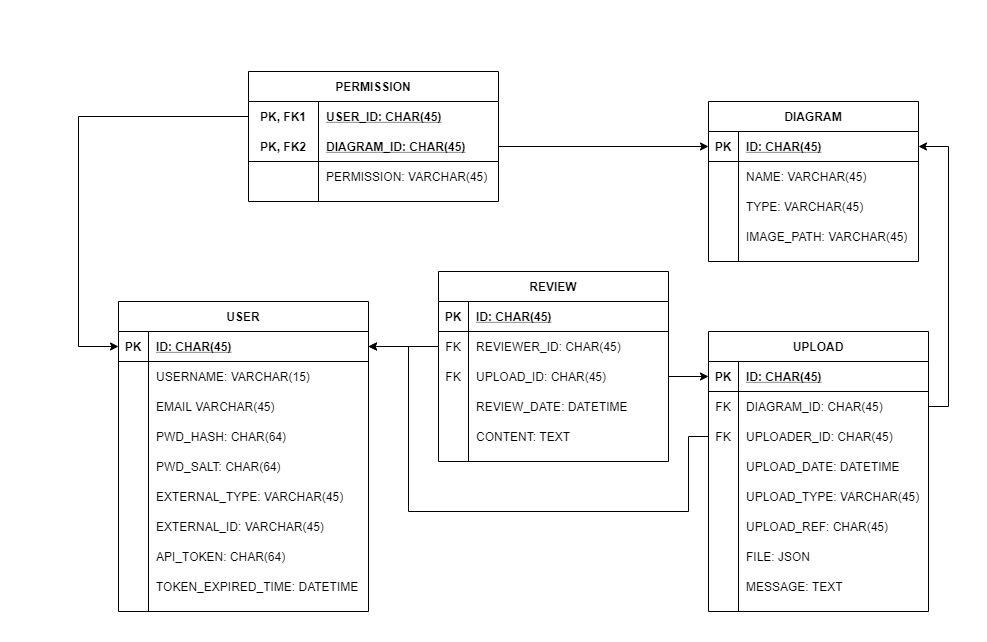
\includegraphics[width=16cm]{Images/App/DB.png}
% \caption{Database Design}
% \end{figure}

% \section{Diagram File Design}
% After having consulted some types of diagrams, we decided to go with .json file since it is widely used and supported by many platforms. It is also able to be stored directly in the My SQL database using JSON data type. Although the size still depends on the server configuration, this is one of the most convenient file types to transfer between the web server and the client devices. The file will have 4 main components: ID, name, an array of symbols, and an array of arrows.

% Figure \ref{fig:jsonfile} shows the json file design used for construct the diagram used in the application.

% \begin{figure}[!b]
% \centering
% 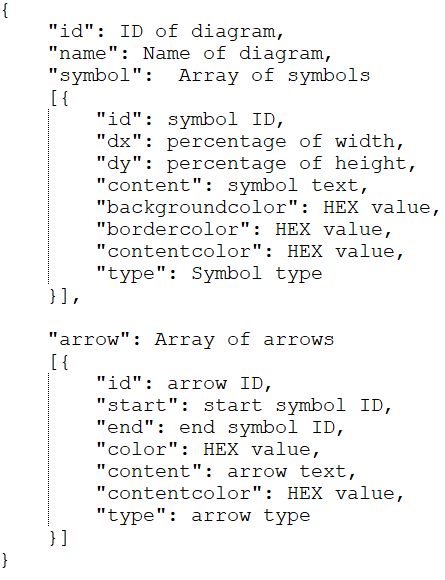
\includegraphics[width=12cm]{Images/App/jsonFile.png}
% \caption{JSON file design}
% \label{fig:jsonfile}
% \end{figure}



% \section{Use case Design}
% \subsection{Use case diagram}
% Figure \ref{fig:usecase} shows the system use case design for the application.

% \begin{figure}[!t]
% \centering
% 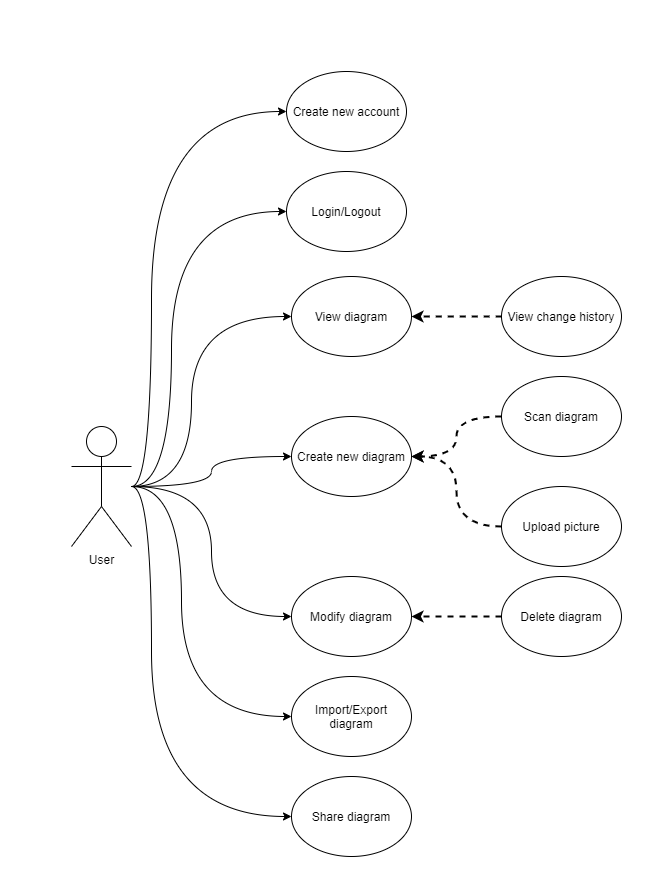
\includegraphics[width=14cm]{Images/App/Usecase.png}
% \caption{Use case Design}
% \label{fig:usecase}
% \end{figure}

% \subsection{Use case detail}
% \begin{table}[b]
% \begin{tabular}{| m{8cm} | m{6cm} |}
% \hline
% Use case name & Table reference\\ \hline
% Login. & Table \ref{Tab:UC-1}\\ \hline
% Sign up. & Table \ref{Tab:UC-2}\\ \hline
% Create new diagram. & Table \ref{Tab:UC-3}\\ \hline
% Scan diagram with camera. & Table \ref{Tab:UC-3.1}\\ \hline
% Scan from image. & Table \ref{Tab:UC-3.2}\\ \hline
% Import file. & Table \ref{Tab:UC-4}\\ \hline
% Export file. & Table \ref{Tab:UC-5}\\ \hline
% Modify diagram. & Table \ref{Tab:UC-6}\\ \hline
% Delete diagram. & Table \ref{Tab:UC-7}\\ \hline
% % Share. & Table \ref{Tab:UC-8}\\ \hline
% % Set permission. & Table \ref{Tab:UC-9}\\ \hline
% % View change history. & Table \ref{Tab:UC-10}\\ \hline
% % Revert. & Table \ref{Tab:UC-11}\\ \hline
% Logout. & Table \ref{Tab:UC-12}\\ \hline
% \end{tabular}
% \captionof{table}{\label{Tab:UCList}Use case List}
% \end{table}

% \begin{table}[]
% \begin{tabular}{| m{4cm} | m{11cm} |}
% \hline
% Use case ID:       & UC-1 \\ \hline
% Use Case Name:     & Login. \\ \hline
% Triggering Event:  & The user open the app and in login screen. \\ \hline
% Brief Description: & System verify user's inputted username and password and go to home screen. \\ \hline
% Actors:            & The user \\ \hline
% Preconditions:     & \begin{itemize}
%     \item Application has internet connection.
%     \item The user has a system account.
%     \item The user has not logged in with Google account.
% \end{itemize} \\ \hline
% Post-conditions:   & \begin{itemize}
%     \item The user is logged in to the system.
%     \item The user is able to perform action that requires the web server.
% \end{itemize} \\ \hline
% Normal flows:      & \begin{enumerate}
%     \item The user opens the app.
%     \item System show login form including username and password.
%     \item The user fill in the form and login.
%     \item System authenticates user.
%     \item The user is logged in and has access to the system.
% \end{enumerate} \\ \hline
% Alternative flows: & \begin{itemize}
%     \item {2a The user has already logged in with Google account}
%     \begin{itemize}
%         \item 2a1 System automatically authenticates user in with Google account.
%         \item 2a3 Use case continue with step 5.
%     \end{itemize}
%     \item {3a The user chooses to log in with Google account}
%     \begin{itemize}
%         \item 3a1 System shows Google logging page.
%         \item 3a2 The user enters essential information.
%         \item 3a3 System receive Google credential.
%         \item 3a4 Use case continue with step 4.
%     \end{itemize}
%     \item {4a The user input an invalid username or password.}
%     \begin{itemize}
%         \item 4a1 System shows an error message.
%         \item 4a2 The user re-input information.
%         \item 4a3 Use case continue with step 4.
%     \end{itemize}
% \end{itemize} \\ \hline
% Exception: & \begin{itemize}
%     \item {2a The user logged in with Google account but the credential is incorrect.}
%     \begin{itemize}
%         \item 2a1 System shows an error message.
%         \item 2a2 Use case continue with step 1.
%     \end{itemize}
% \end{itemize} \\ \hline
% \end{tabular}
% \captionof{table}{\label{Tab:UC-1} Use case: Login.}
% \end{table}

% \begin{table}[]
% \begin{tabular}{| m{4cm} | m{11cm} |}
% \hline
% Use case ID:       & UC-2 \\ \hline
% Use Case Name:     & Sign up. \\ \hline
% Triggering Event:  & The user choose ''Sign up'' in login screen. \\ \hline
% Brief Description: & The user want to create a new system account. \\ \hline
% Actors:            & The user \\ \hline
% Preconditions:     & \begin{itemize}
%     \item The user has an email account.
%     \item Application has internet connection.
%     \item The user has not logged in the system.
% \end{itemize} \\ \hline
% Post-conditions:   & \begin{itemize}
%     \item A new account is registered in the system with distinct user name.
%     \item The user is logged in and has access to system function.
% \end{itemize} \\ \hline
% Normal flows:      & \begin{enumerate}
%     \item The user open the app and choose ''Sign up'' function.
%     \item System show the register form including username, email, password.
%     \item The user enters the essential information.
%     \item System check if all of the information are valid and create a new account.
%     \item System authenticates user.
%     \item The user is logged in and has access to the system.
% \end{enumerate} \\ \hline
% Alternative flows: & \begin{itemize}
%     \item {4a The user input an invalid username or password.}
%     \begin{itemize}
%         \item 4a1 System shows an error message.
%         \item 4a2 The user re-input information.
%         \item 4a3 Use case continue with step 4.
%     \end{itemize}
%     \item {4a The user input an already existed username.}
%     \begin{itemize}
%         \item 4a1 System shows an error message and provide login option.
%         \item 4a2 The user choose login.
%         \item 4a3 Use case continue with table \ref{Tab:UC-1}.
%     \end{itemize}
% \end{itemize} \\ \hline
% Exception: & N/A\\ \hline
% \end{tabular}
% \captionof{table}{\label{Tab:UC-2} Use case: Sign up.}
% \end{table}

% \begin{table}[]
% \begin{tabular}{| m{4cm} | m{11cm} |}
% \hline
% Use case ID:       & UC-3 \\ \hline
% Use Case Name:     & Create new diagram. \\ \hline
% Triggering Event:  & The user wants to create a new diagram. \\ \hline
% Brief Description: & At home screen, user wants to create a new diagram. \\ \hline
% Actors:            & The user \\ \hline
% Preconditions:     &  \\ \hline
% Post-conditions:   & \begin{itemize}
%     \item A diagram is detected.
%     \item A new temporary file is created.
% \end{itemize} \\ \hline
% Normal flows:      & \begin{enumerate}
%     \item The user opens the app.
%     \item The user chooses to create a blank diagram.
%     \item The user input diagram name.
%     \item System show file browser with default saving location.
%     \item The user chooses location to save diagram.
%     \item System create new file in storage and go to modify page.
% \end{enumerate} \\ \hline
% Alternative flows: & \begin{itemize}
%     \item {2a The user choose to scan a new diagram directly.}
%     \begin{itemize}
%         \item 2a1 Use case continue with table \ref{Tab:UC-3.1}.
%         \item 2a2 Use case continue with step 3.
%     \end{itemize}
%     \item {2b The user choose to scan a new diagram from image.}
%     \begin{itemize}
%         \item 2a1 Use case continue with table \ref{Tab:UC-3.2}.
%         \item 2a2 Use case continue with step 3.
%     \end{itemize}
% \end{itemize} \\ \hline
% Exception: & \begin{itemize}
%     \item {3a The user do not input diagram name.}
%     \begin{itemize}
%         \item 3a1 System uses default name (New Diagram).
%         \item 3a2 Use case continue with step 4.
%     \end{itemize}
%     \item {3b The user delete default name and leave name blank.}
%     \begin{itemize}
%         \item 3b1 System shows an error alert and let user try again.
%         \item 3b2 Use case continue with step 3.
%     \end{itemize}
%     \item {5a if the app has not been granted access to storage.}
%     \begin{itemize}
%         \item 5a1 System shows access permission notification.
%         \item 5a2 The user allow storage permission.
%         \item 5a3 Use case continue with step 6.
%     \end{itemize}
%     \item {5b If system cannot create a new file.}
%     \begin{itemize}
%         \item 5b1 System show error and return to home screen.
%         \item 5b2 Use case stop
%     \end{itemize}
% \end{itemize} \\ \hline
% \end{tabular}
% \captionof{table}{\label{Tab:UC-3} Use case: Create new diagram.}
% \end{table}

% \begin{table}[]
% \begin{tabular}{| m{4cm} | m{11cm} |}
% \hline
% Use case ID:       & UC-3.1 \\ \hline
% Use Case Name:     & Scan diagram with camera. \\ \hline
% Triggering Event:  & The user wants to scan a new diagram with camera. \\ \hline
% Brief Description: & The user chooses to scan device camera in create options. \\ \hline
% Actors:            & The user \\ \hline
% Preconditions:     & \\ \hline
% Post-conditions:   & \begin{itemize}
%     \item A diagram is detected.
% \end{itemize} \\ \hline
% Normal flows:      & \begin{enumerate}
%     \item The user takes a picture of the diagram.
%     \item The user adjusts the boundary of the diagram.
%     \item System shows result.
%     \item The user chooses “Done”. 
%     \item System continue with previous use case.
% \end{enumerate} \\ \hline
% Alternative flows: & \begin{itemize}
%     \item {2a The user want to retake the picture.}
%     \begin{itemize}
%         \item Use case continue with step 1.
%     \end{itemize}
% \end{itemize} \\ \hline
% Exception: & \begin{itemize}
%     \item {3a If there is no diagram detected.}
%     \begin{itemize}
%         \item 3a1 System show an error.
%         \item 3a2 The user choose to retake the picture.
%         \item 3a3 Use case continue with step 1.
%     \end{itemize}
% \end{itemize} \\ \hline
% \end{tabular}
% \captionof{table}{\label{Tab:UC-3.1} Use case: Scan diagram with camera.}
% \end{table}

% \begin{table}[]
% \begin{tabular}{| m{4cm} | m{11cm} |}
% \hline
% Use case ID:       & UC-3.2 \\ \hline
% Use Case Name:     & Scan from image. \\ \hline
% Triggering Event:  & The user clicks on “Scan from image” button in create options. \\ \hline
% Brief Description: & The user chooses to scan a new diagram from an image.\\ \hline
% Actors:            & The user \\ \hline
% Preconditions:     & N/A\\ \hline
% Post-conditions:   & \begin{itemize}
%     \item A diagram is detected.
% \end{itemize} \\ \hline
% Normal flows:      & \begin{enumerate}
%     \item System shows the storage browser.
%     \item The user chooses a picture.
%     \item System shows the full picture.
%     \item The user adjusts the boundary of the diagram.
%     \item The user chooses “Done”. 
%     \item System save the result and continue with previous use case.
% \end{enumerate} \\ \hline
% Alternative flows: & N/A\\ \hline
% Exception: & \begin{itemize}
%     \item {2a The user chooses a file that is not a picture.}
%     \begin{itemize}
%         \item 2a1 System show a warning
%         \item 2a2 The user choose to cancel.
%         \item 2a3 Use case stop.
%     \end{itemize}
%     \item {3a there is no diagram detected.}
%     \begin{itemize}
%         \item 3a1 System show an error.
%         \item 3a2 The user choose to retake the picture.
%         \item 3a3 Use case continue with step 1.
%     \end{itemize}
% \end{itemize} \\ \hline
% \end{tabular}
% \captionof{table}{\label{Tab:UC-3.2} Use case: Scan from image.}
% \end{table}

% \begin{table}[]
% \begin{tabular}{| m{4cm} | m{11cm} |}
% \hline
% Use case ID:       & UC-4 \\ \hline
% Use Case Name:     & Import file. \\ \hline
% Triggering Event:  & The user clicks on “Import file” button. \\ \hline
% Brief Description: & The user is in home page and want to import a file in storage to the app. \\ \hline
% Actors:            & The user \\ \hline
% Preconditions:     & N/A\\ \hline
% Post-conditions:   & \begin{itemize}
%     \item A new diagram is imported and show in home screen.
% \end{itemize} \\ \hline
% Normal flows:      & \begin{enumerate}
%     \item The user chooses to import from local storage.
%     \item System shows the storage browser.
%     \item The user chooses a file.
%     \item System save file location and show new diagram in home screen.
% \end{enumerate} \\ \hline
% Alternative flows: & \begin{itemize}
%     \item {2a The user choose to import from Google drive.}
%     \begin{itemize}
%         \item 2a1 The user login to Google Drive.
%         \item 2a2 System shows Google Drive file browser.
%         \item 2a3 Use case continue with step 3.
%     \end{itemize}
% \end{itemize} \\ \hline
% Exception: & \begin{itemize}
%     \item {3a The user chooses a file that is compatible or not accessible.}
%     \begin{itemize}
%         \item 3a1 System show a warning.
%         \item 3a2 The user choose to cancel.
%         \item 3a3 Use case stop.
%     \end{itemize}
% \end{itemize} \\ \hline
% \end{tabular}
% \captionof{table}{\label{Tab:UC-4} Use case: Import file.}
% \end{table}

% \begin{table}[]
% \begin{tabular}{| m{4cm} | m{11cm} |}
% \hline
% Use case ID:       & UC-5 \\ \hline
% Use Case Name:     & Export file. \\ \hline
% Triggering Event:  & The user clicks on “Export” button in diagram options. \\ \hline
% Brief Description: & The user wants to export a diagram. \\ \hline
% Actors:            & The user \\ \hline
% Preconditions:     & N/A\\ \hline
% Post-conditions:   & \begin{itemize}
%     \item A new diagram file is created.
% \end{itemize} \\ \hline
% Normal flows:      & \begin{enumerate}
%     \item The user selects a diagram and choose “Export”.
%     \item The user selects “Export as an image”.
%     \item The user chooses save location and select “Done”.
%     \item System create an image of selected diagram.
% \end{enumerate} \\ \hline
% Alternative flows: & \begin{itemize}
%     \item {2a The user select “Export as .pdf file”.}
%     \begin{itemize}
%         \item 2a1 The user chooses save location and select “Done”.
%         \item 2a2 System create an pdf file of selected diagram.
%         \item 2a3 Use case stop.
%     \end{itemize}
%     \item {2b The user select “Export as .drawio file”.}
%     \begin{itemize}
%         \item 2b1 The user chooses save location and select “Done”.
%         \item 2b2 System create a drawio file of selected diagram.
%         \item 2b3 Use case stop.
%     \end{itemize}
% \end{itemize} \\ \hline
% Exception: & \begin{itemize}
%     \item {3a If the diagram is blank, show a warning and allow user to cancel.}
%     \begin{itemize}
%         \item 3a1 The user cancel the operation.
%         \item Use case stop.
%     \end{itemize}
%     \item {3b if the app has not been granted access to storage.}
%     \begin{itemize}
%         \item 3b1 System shows access permission notification.
%         \item 3b2 The user allow storage permission.
%         \item 3b3 Use case continue with step 4.
%     \end{itemize}
% \end{itemize} \\ \hline
% \end{tabular}
% \captionof{table}{\label{Tab:UC-5} Use case: Export file.}
% \end{table}

% \begin{table}[]
% \begin{tabular}{| m{4cm} | m{11cm} |}
% \hline
% Use case ID:       & UC-6 \\ \hline
% Use Case Name:     & Modify diagram. \\ \hline
% Triggering Event:  & The user clicks on “Modify” button in diagram options. \\ \hline
% Brief Description: & The user wants to modify a diagram showed in home screen. \\ \hline
% Actors:            & The user \\ \hline
% Preconditions:     & N/A\\ \hline
% Post-conditions:   & \begin{itemize}
%     \item All changes is recorded and uploaded to server.
% \end{itemize} \\ \hline
% Normal flows:      & \begin{enumerate}
%     \item The user selects a diagram.
%     \item System shows diagram options.
%     \item The user selects “Modify”.
%     \item System go to modify page.
%     \item The user performs changes to the diagram.
%     \item The user selects “Save”.
%     \item System saves all changes and go back to home screen
% \end{enumerate} \\ \hline
% Alternative flows: & \begin{itemize}
%     \item {6a The user select ''Discard''.}
%     \begin{itemize}
%         \item 6a1 Systems show confirm message.
%         \item 6a2 The user select ''Yes''.
%         \item 6a3 Systems delete all changes and return to home screen.
%         \item 6a4 Use case stop.
%     \end{itemize}
% \end{itemize} \\ \hline
% Exception: & \begin{itemize}
%     \item {7a System cannot save file.}
%     \begin{itemize}
%         \item 7a1 System show saving error.
%         \item 7a2 The user selects cancel.
%         \item 7a3 Systems delete all changes and return to home screen.
%         \item 7a4 Use case stop.
%     \end{itemize}
%     \item {7b if the app has not been granted access to storage.}
%     \begin{itemize}
%         \item 7b1 System shows access permission notification.
%         \item 7b2 The user allow storage permission.
%         \item 7b3 Use case continue with step 4.

%     \end{itemize}
% \end{itemize} \\ \hline
% \end{tabular}
% \captionof{table}{\label{Tab:UC-6} Use case: Modify diagram.}
% \end{table}

% \begin{table}[]
% \begin{tabular}{| m{4cm} | m{11cm} |}
% \hline
% Use case ID:       & UC-7 \\ \hline
% Use Case Name:     & Delete Diagram. \\ \hline
% Triggering Event:  & The user choose ''Delete'' in diagram options. \\ \hline
% Brief Description: & The user want to delete a diagram from home screen. \\ \hline
% Actors:            & The user \\ \hline
% Preconditions:     & \begin{itemize}
%     \item The user is in home screen.
%     \item The user is the owner of the diagram.
%     \item The diagram is no longer shared with any other user.
% \end{itemize} \\ \hline
% Post-conditions:   & \begin{itemize}
%     \item The diagram is deleted in the database.
% \end{itemize} \\ \hline
% Normal flows:      & \begin{enumerate}
%     \item The user select a diagram, chooses ''Delete'' option.
%     \item System shows a warning message.
%     \item The user confirms to delete.
%     \item System deletes the diagram and shows the result message.
% \end{enumerate} \\ \hline
% Alternative flows: & \begin{itemize}
%     \item {4a The diagram is still shared to other users.}
%     \begin{itemize}
%         \item 4a1 System show error message and provide ''provoke all permission'' option.
%         \item 4a2 The user confirm.
%         \item 4a3 System delete all of share permission.
%         \item 4a4 Use case continue with step 4.
%     \end{itemize}
% \end{itemize} \\ \hline
% Exception: & \begin{itemize}
%     \item {4a The user is not the owner of the diagram.}
%     \begin{itemize}
%         \item 4a1 System show error message.
%         \item 4a2 Use case stops.
%     \end{itemize}
% \end{itemize} \\ \hline
% \end{tabular}
% \captionof{table}{\label{Tab:UC-7} Use case: Delete Diagram.}
% \end{table}

% \begin{table}[]
% \begin{tabular}{| m{4cm} | m{11cm} |}
% \hline
% Use case ID:       & UC-8 \\ \hline
% Use Case Name:     & Share. \\ \hline
% Scenario:          & . \\ \hline
% Triggering Event:  & . \\ \hline
% Brief Description: & . \\ \hline
% Actors:            & The user \\ \hline
% Preconditions:     & \\ \hline
% Post-conditions:   & \begin{itemize}
%     \item .
% \end{itemize} \\ \hline
% Normal flows:      & \begin{enumerate}
%     \item 
% \end{enumerate} \\ \hline
% Alternative flows: & \begin{itemize}
%     \item {.}
%     \begin{itemize}
%         \item 
%     \end{itemize}
% \end{itemize} \\ \hline
% Exception: & \begin{itemize}
%     \item {.}
%     \begin{itemize}
%         \item 
%     \end{itemize}
% \end{itemize} \\ \hline
% \end{tabular}
% \captionof{table}{\label{Tab:UC-8} Share.}
% \end{table}

% \begin{table}[]
% \begin{tabular}{| m{4cm} | m{11cm} |}
% \hline
% Use case ID:       & UC-9 \\ \hline
% Use Case Name:     & Set permission. \\ \hline
% Scenario:          & . \\ \hline
% Triggering Event:  & . \\ \hline
% Brief Description: & . \\ \hline
% Actors:            & The user \\ \hline
% Preconditions:     & \\ \hline
% Post-conditions:   & \begin{itemize}
%     \item .
% \end{itemize} \\ \hline
% Normal flows:      & \begin{enumerate}
%     \item 
% \end{enumerate} \\ \hline
% Alternative flows: & \begin{itemize}
%     \item {.}
%     \begin{itemize}
%         \item 
%     \end{itemize}
% \end{itemize} \\ \hline
% Exception: & \begin{itemize}
%     \item {.}
%     \begin{itemize}
%         \item 
%     \end{itemize}
% \end{itemize} \\ \hline
% \end{tabular}
% \captionof{table}{\label{Tab:UC-9} Set permission.}
% \end{table}

% \begin{table}[]
% \begin{tabular}{| m{4cm} | m{11cm} |}
% \hline
% Use case ID:       & UC-10 \\ \hline
% Use Case Name:     & View change history. \\ \hline
% Scenario:          & . \\ \hline
% Triggering Event:  & . \\ \hline
% Brief Description: & . \\ \hline
% Actors:            & The user \\ \hline
% Preconditions:     & \\ \hline
% Post-conditions:   & \begin{itemize}
%     \item .
% \end{itemize} \\ \hline
% Normal flows:      & \begin{enumerate}
%     \item 
% \end{enumerate} \\ \hline
% Alternative flows: & \begin{itemize}
%     \item {.}
%     \begin{itemize}
%         \item 
%     \end{itemize}
% \end{itemize} \\ \hline
% Exception: & \begin{itemize}
%     \item {.}
%     \begin{itemize}
%         \item 
%     \end{itemize}
% \end{itemize} \\ \hline
% \end{tabular}
% \captionof{table}{\label{Tab:UC-10} View change history.}
% \end{table}

% \begin{table}[]
% \begin{tabular}{| m{4cm} | m{11cm} |}
% \hline
% Use case ID:       & UC-11 \\ \hline
% Use Case Name:     & Revert.. \\ \hline
% Triggering Event:  & User wants to revert back to the previous version of the diagram. \\ \hline
% Brief Description: & User choose ''Revert'' on the version in the history change. \\ \hline
% Actors:            & The user \\ \hline
% Preconditions:     & \begin{itemize}
%     \item User is the owner or has ''Can edit'' permission.
%     \item The selected version is not the current one.
% \end{itemize} \\ \hline
% Post-conditions:   & \begin{itemize}
%     \item A reverted upload is sent.
% \end{itemize} \\ \hline
% Normal flows:      & \begin{enumerate}
%     \item 
% \end{enumerate} \\ \hline
% Alternative flows: & \begin{itemize}
%     \item {.}
%     \begin{itemize}
%         \item 
%     \end{itemize}
% \end{itemize} \\ \hline
% Exception: & \begin{itemize}
%     \item {.}
%     \begin{itemize}
%         \item 
%     \end{itemize}
% \end{itemize} \\ \hline
% \end{tabular}
% \captionof{table}{\label{Tab:UC-11} Revert..}
% \end{table}

% \begin{table}[]
% \begin{tabular}{| m{4cm} | m{11cm} |}
% \hline
% Use case ID:       & UC-12 \\ \hline
% Use Case Name:     & Logout. \\ \hline
% Triggering Event:  & The user is done using the app and want to logout. \\ \hline
% Brief Description: & The user chooses ''Log out'' and ends their logging session. \\ \hline
% Actors:            & The user \\ \hline
% Preconditions:     & \begin{itemize}
%     \item The user is logged in.
% \end{itemize} \\ \hline
% Post-conditions:   & \begin{itemize}
%     \item The user is logged out.
% \end{itemize} \\ \hline
% Normal flows:      & \begin{enumerate}
%     \item The user choose ''Option'' and ''Logout''.
%     \item System logs user out and invalidates the API key.
%     \item System redirects to login screen.
% \end{enumerate} \\ \hline
% Alternative flows: & N/A \\ \hline
% Exception: & N/A \\ \hline
% \end{tabular}
% \captionof{table}{\label{Tab:UC-12} Use case: Logout.}
% \end{table}